\section{Расширяемы протокол аутентификации (EAP)}

Процесс аутентификации EAP происходит следующим образом:

\begin{enumerate}
\item Аутентификатор отправляет запрос аутентификации пиру. Запрос содержит поле ``Type'' в котором указывается что запрашивается. Поле ``Type'' может сообщать о запросах: идентификации, MD5-запрос, и т.д. MD5-запрос близок к описанию из протокола CHAP аутентификации (RFC1994). Обычно, аутентификатор отправляет запрос идентификатора для начала процедуры аутентификации; однако такой запрос не обязателен для протокола и может быть пропущен. Например такой запрос не требуется, если идентификатор определяется поротом, к которому подключен пир (выделенная линия, специализированный свич или диал-ап порт), или другим методом (идентификатор станции свящи, MAC-адрес, и т.д.)
\item Пир посылает ответ на корректны запрос. Как и запрос, ответ содержит поле ``Type'' которое показывает тип запроса.
\item Аутентификатор отправляет дополнительный запрос и пир отвечает на него. Такой обмен происходит столько раз, сколько необходимо для процесса. EAP жестко регламантированный протокол, так что новые запросы, не отправляются пока не придет корректный ответ на предыдущщий запрос. Аутентификатор отвечает за повторную отправку запросов, данный механизм описан в пункте 4.1. После отправки некоторого количества повторных запросов Аутентификатор ДОЛЖЕН завершить EAP передачу данных. При этом Аутентификатор НЕ ДОЛЖЕН отправлять пакеты ``Success'' или ``Failure'' при повторной отправке пакета или когда не удается получить ответ от пира.
\item Обмен продолжаеься до тех пор, пока Аутентификатор не сможет аутентифицировать пира (неприемлемый ответ на один или несколько запросов), в этом случае Аутентификатор ДОЛЖЕН передать сообщение ``EAP Failure'' (Код 4). Так же обмен продолжается до успешной аутентификации пира, в этом случае Аутентификатор ДОЛЖЕН передать сообщение ``EAP Success'' (Код 3).
\end{enumerate}

Преимущества:

\begin{itemize}
\item EAP может поддерживать одновременно несколько протоколов аутентификации без предварительного соглашения о том, какой именно будет использоваться;
\item Сервер сетевого доступа (NAS) (например свич или точка доступа) не знают какой метод аутентификации используется и МОЖЕТ являться прозрачным шлюзом для базового сервера аутентификации. Поддержка сквозного режима является необязательной. Аутентификатор МОЖЕТ аутентифицировать локальные пиры, в то же время выступая шлюзом для не локальных пиров и методов аутентификации реализуемых не локально.
\item Отделение аутентификатора от базового сервера аутентификации упрощает управление полономочиями и политикой безопасности.
\end{itemize}

Недостатки:

\begin{itemize}
\item При использовании PPP, EAP необходимо добавить новый тип аутентификации - PPP LCP и изменить реализацию PPP для использования этого протокола. Это так же откланяет аутентификацию по PPP от спецификации LCP. Так же точки доступа и свичи должны поддерживать реализацию IEEE-802.1X для использования EAP.
\item Если аутентификатор отделяется от базового сервера аутентификации, то усложняется анализ механизмов безопасности и появляется проблема распределения ключей.
\end{itemize}

\subsection{Поддержка последовательностей}

В рамках EAP МОЖЕТ использоваться последовательность методов. Типичным премером этого может быть запрос идентификатора при использовании MD5-вызова. Тем не менее Аутентификатор и пир должны использовать только один метод аутентификации (Type 4 или выше) во время процедуры аутентификации в конце которой Аутнетификатор ДОЛЖЕН отправить ``Success'' или ``Failure''.

После того как пир отправил ответ того же типа что и предыдущий запрос, Аутентификатор НЕ ДОЛЖЕН отправлять другие запросы до окончания процедуры аутентификации (кроме запросов уведомления) и НЕ ДОЛЖЕН отправлять запросы на дополнительные методы аутентификации после окончания выолнения первоначального метода аутентификации; пир не должен реагировать на такие запросы и отбрасывать их как невалидные. Таким образом перезапросы аутентификации не поддерживаются.

Пир не должен отправлять Nak (Наследования или Расширения) в ответ на запрос после того как отправил non-Nak ответ на запрос. Такие поддельные EAP покеты могут быть отправлены атакующим. Аутентификатор при получении неожиданного Nak ответа ДОЛЖЕН его проигнорировать и сделать запись об этом в журнал событий.

Множественные методы аутентификации EAP в рамках одного сеанса не используются так как такие методы уязвимы к атакам ``человек посередине'' (Пункт 7.4) и не совместимы с существующими реализациями.

Если используется метод аутентификации, но внутри него используются другие методы (например тунелирование), то запрет на множественные методы аутентификации не применяется. Такие методы можно рассматривать как один метод аутентификации. Если пир не поддерживает тунелирование, то совместимость может быть обеспечена при помощи начального Nak-запроса (Наследования или Расширения). Для обеспечения должного уровня безопасности методы тунелирования должны иметь механизмы защиты от атака типа ``человек посередине''.

\subsection{Модель мультиплексирования EAP}

Концептуально, реализация EAP состоит из следующих компонентов:

\begin{itemize}
\item Нижний уровень. Нижний уровень отвечает за передачу и прием кадров EAP между пиром и Аутентификатором. EAP запускается поверх различных уровней, таких как PPP, проводные сети 802 (IEEE-802-1X), беспроводные (IEEE 802.11), UDP (L2TP (RFC2661) и IKEv2 (IKEv2)) и TCP (PIC). Работа нижнего уровня описывается в пункте 3.
\item Уровень EAP. Уровень EAP передает и принимает EAP пакеты при помощи нижнего уровня, осуществляет обноружения дублирования и повтор отправки, а так же передает и принимает EAP сообщения с уровня ``Пир и Аутентификатор EAP''
\item Уровень пира и Аутентификатора EAP. Основываясь на поле ``Code'' Уровень EAP демультиплексирует входящие EAP пакеты в Уровень пира и Аутентификатора EAP. Обычно реализация EAP на устройстве поддерживает функционал либо пира, либо Аутентификатора, но возможно что хост действует как EAP пир и Аутентификатор. При такой реализации на устройстве будут присутствовать слои пира и Аутентификатора.
\item Уровень метода EAP. Уровень метода EAP реализует алгоритмы аутентификации и получает и отправляет сообщения EAP при помощи уровня пира и Аутентификатора EAP. Сам EAP не поддерживает фрагментацию данных, за это отвечают EAP методы, описанные в пункте 5.
\end{itemize}

Модель мультиплексирования EAP представлена на рисунке \ref{img:1}. Стоит отметить, что нет требований к реализации, по которым необходимо придерживаться данной модели, при условии что поведение реализации соответствует требованиям.

\begin{figure}[h]
\center{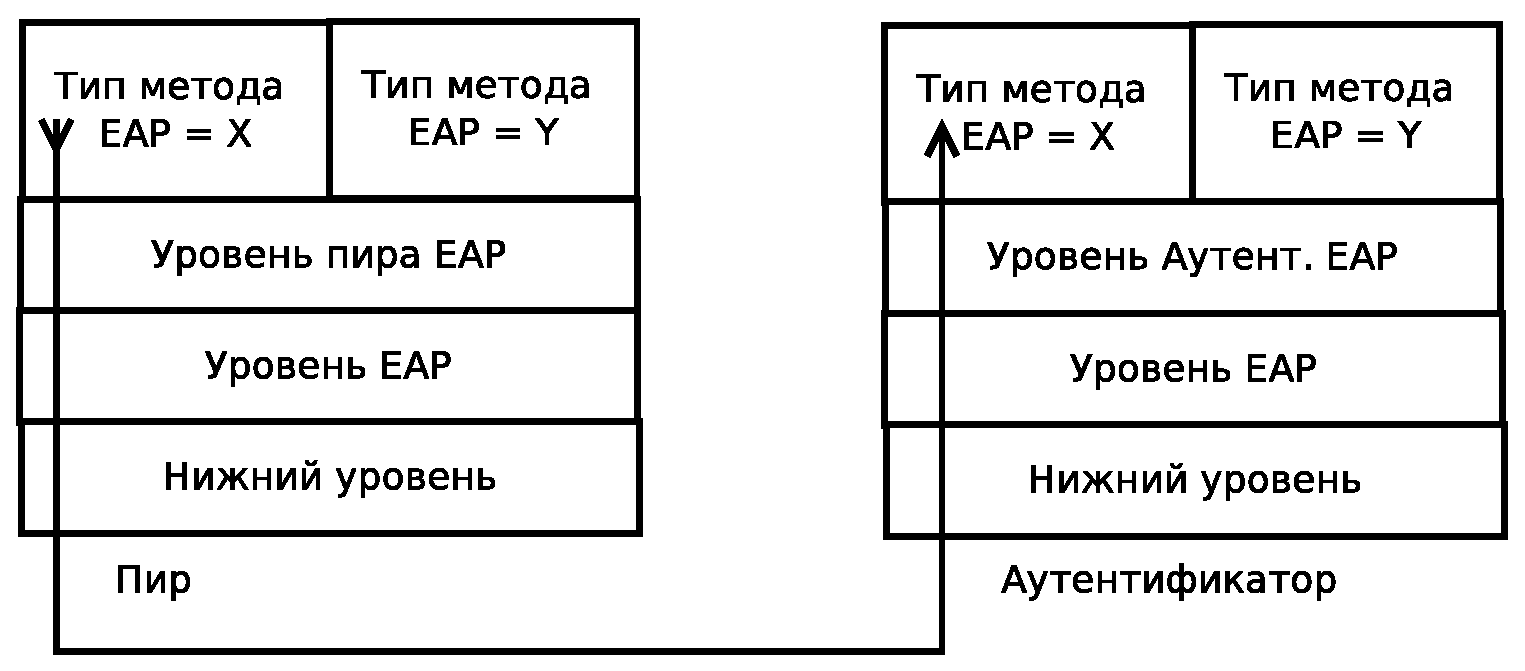
\includegraphics[width=0.9\linewidth]{./pictures/1}}
\caption{Модель мултиплексирования EAP}
\label{img:1}
\end{figure}

В EAP поле ``Code'' похоже на номер протокола в IP. Предполагается, что EAP демультиплексирует входящие пакеты в соответствии с полем ``Code''. Поступивший EAP пакет с полем ``Code'' = 1 (Request), 3 (Success) и 4 (Failure) передаются уровнем EAP на уровень пира EAP если данный слой реализован. EAP пакеты с полем ``Code'' = 2 (Response) передаются уровню Аутентификатора EAP если слой реализован.

В EAP поле ``Type'' похоже на номер порта в UDP или TCP. Предполагается, что уровень пира и Аутентификатора EAP демультиплексирует входящие EAP пакеты в соответствии с их типом (значением поля ``Type'') и передает их методу EAP соответствующего типа. Реализация EAP метода на хосте может указать что она принимает пакеты от уровня пира, Аутентификатора или от двух уровней сразу, взависимости от того, какую роль (роли) она подерживает.

Поскольку методы аутентификации EAP могут запросить идентификатор, реализация ДОЛЖНА поддерживать запрос и ответ идентификатора, доступные методам аутентификации (``Type'' 4 или больше) в дополнении к методу Idetity. Значения поля ``Type'' для метода Identity описаны в пункте 5.1.

Ответ на Notification запрос используется только для того, что бы пир уведомил о получении такого запроса, а не для подтверждения обработки запроса или отображения сообщений для пользователя. Не предполагается, что содержимое Notification запроса и ответа возможно получить другими методами. Поле ``Type'' для Notification запроса описываются в пункте 5.2.

Nak (``Type'' = 3) или расширенный Nak (``Type'' = 254) используются методами согласования. Пиры отвечают на инициализирующий EAP запрос ответом с недопустимым полем ``Type'' = 3 (Nak) или 4 (расширенный Nak). Не прелполагается, что содержимое Nak ответов можно получить другими методами. Поле ``Type'' для Nak описываются в пункте 5.3.

EAP пакеты с полем ``Code'' Success или Failure не включают в себя поле ``Type'' и не передается EAP методам. Success и Failure описаны в пункте 4.2.

Исходя из этого, сообщения с Success, Failure и Nak ответами и Notification запросами/ответами НЕ ДОЛЖНЫ использоваться для передачи данных, предназначенных другим методам EAP.

\subsection{Режим ретрансляции}

При работе устройства в режиме ретрансляции, Аутентификатор производит проверку ``Code'', идентификатор и длину поля как описано в пункте 4.1. При работе в данном режиме EAP пакеты, полученные от пира, направляются на уровень Аутентификатора базовому серверу аутентификации; пакеты, полученные от базового сервера аутентификации передаются пиру, которому они предназначены.

Хост, получающий EAP пакет, может сделать с ним тир вещи: обработать его, проигнорировать его, передать его. Решение о передаче пакета дальше основывается на ищучении поля ``Code'', идентификатора и длины поля. Реализация режима ретрансляции ДОЛЖНА быть способна передавать EAP пакеты с ``Code'' = 2 (Запрос), полученные от пиров, на базовый сервер аутентификации. Так же ДОЛЖНЫЕ передаваться пакеты от базового сервера аутентификации к пиру, если EAP пакет имеет поле ``Code'' = 1 (Запрос), 3 (Success) и 4 (Failure).

Если реализация Аутентификатора не поддерживет один или несколько методов аутентификации локально, то заголовок уровня методов EAP (Type, Type-Data), не рассматривается при принятии решения о ретрансляции. Если Аутентификатор поддерживат методы аутентификации, то для принятия решения обрабатывать пакет или передавать дальше МОЖЕТ рассматриваться значение поля ``Type''. Соответственно реализация режима ретрансляции ДОЛЖНА по умолчанию передавать все EAP пакеты, не зависимо от их поля ``Type''.

Пакет EAP, полученный с полем ``Code'' = 1 (Запрос), 3 (Success) и 4 (Failure) демультиплексируются слоем EAP и передаются слою пира. Поэтому, если реализация уровня пира не поодерживается, то такие пакеты отбрасываются. Точно так же, пакеты EAP с полем ``Code'' = 2 (Ответ) демультиплексируются слоем EAP и передаются слою Аутентификатора. Следовательно, если реализация уровня Аутентификатора не поддерживается, то такие пакеты отбрасываются. Режим ретрансляции не описывается в данном документе и не поддерживатся протоколами AAA, такими как RADIUS (RFC3579) и Diameter (DIAM-EAP).

Модель передачи пакетов представлена на рисунке \ref{img:2}.

\begin{figure}[h]
\center{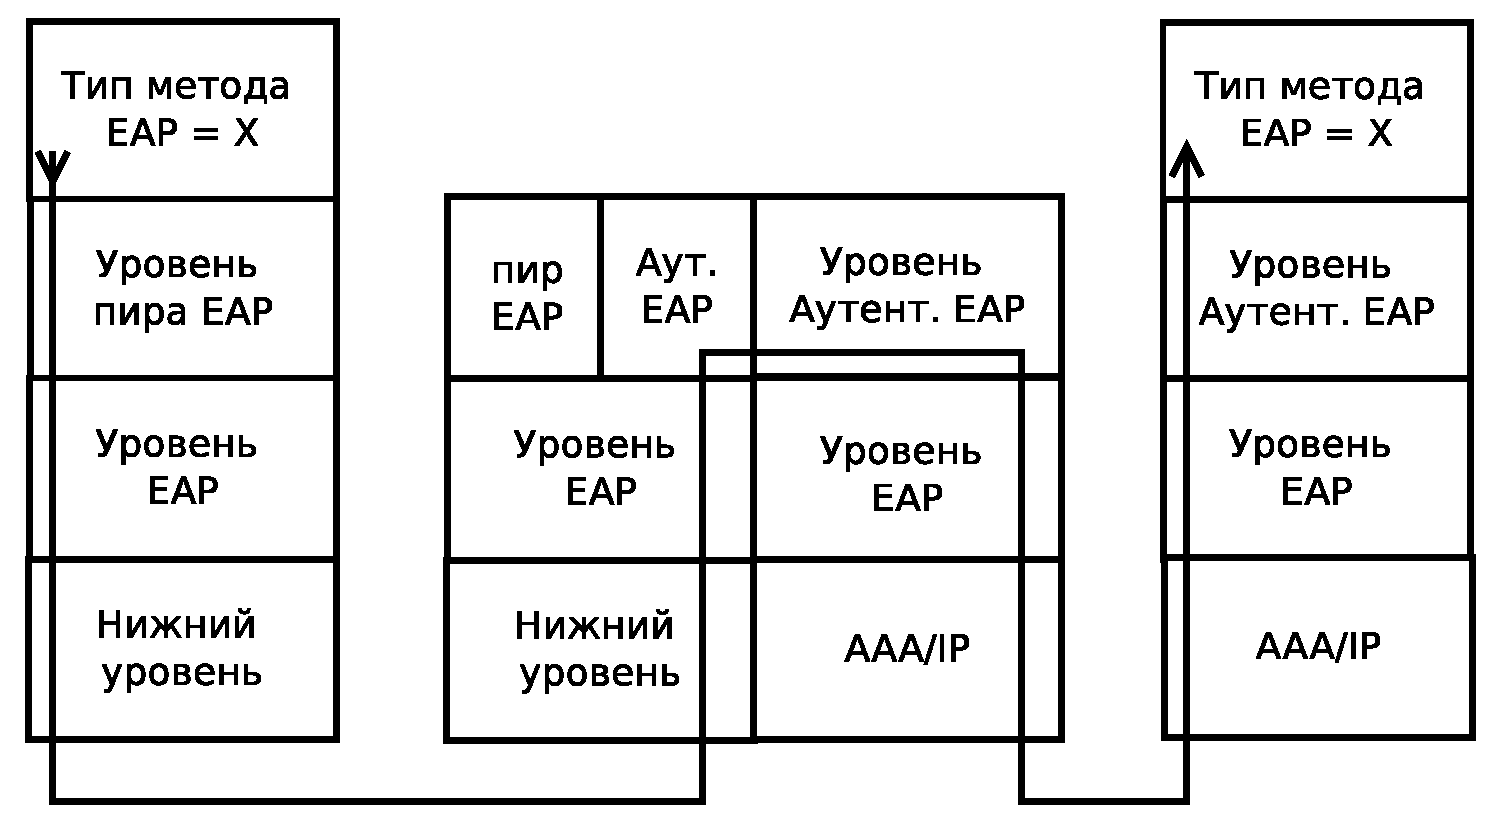
\includegraphics[width=0.9\linewidth]{./pictures/2}}
\caption{Режим ретрансляции}
\label{img:2}
\end{figure}

Для сессий, в которых Аутентификатор выступает в роли ретранслятор, он ДОЛЖЕН определить результат аутентификации, основанный исключительно на индикации Accept/Reject, отправляемой базовым сервером аутентификации; результат НЕ ДОЛЖЕН определятся по содержимому EAP пакетов, передаваемых вместе с индикацией Accept/Reject, или при отсутствии таковой по инкапсулируемому EAP пакету.

\subsection{Операции точка-точка (одноранговые операции)}

Поскольуо EAP является протоколом типа "точка-точка", независимая и одновременная аутентификация может проходить в обратном направлении (зависит от возможностей нижнего уровня). Оба участника сессии могут действовать одновременно как Аутентификатор и пир. В этом случае необходимо что бы оба участника сессии имели реализацию и уровня аутентификатори, и уровня пира. Кроме того реализация EAP у обоих участников должна поддерживать функции и аутентификатора, и пира.

Хотя EAP поддерживает методы точка-точка, некоторые реализации EAP, методы, AAA-протоколы и канальный уровень могут не поддерживать такие методы. Некоторые EAP методы могут поддерживать асимметричную аутентификацию с различными учетными данными для аутентификации пира и Аутентификатора. Хосты поддерживающие операции "точка-точка" при работе с такими методами необходимо снабжать учетными данными обоих типов.

Например EAP-TLS (RFC2716) является клиент-серверным протоколом, в котором, как правило, для клиента и сервера используются сертификаты различной структуры. Это означает, что хост, поддерживающий аутентификацию "точка-точка" при помощи EAP-TLS должен иметь реализацию слоя Аутентификатора и слоя пира, поддерживать обе роли в реализации EAP-TLS и иметь соответствующий сертификат для каждой роли.

AAA протоколы такие как RADIUS/EAP (RFC3579) и Diameter EAP (DIAM-EAP) поддерживают только "сквозную" аутентификацию. Как описано в RFC3579 пункт 2.6.2, RADIUS-сервер отечает на запросы доступа инкапсуляцией в пакеты EAP-запроса, Success или Failure индикации Access-Reject. Поэтому "сквозная" связь не поддерживается.

Даже в тех случаях когда используется метод взаимной аутентификации и результирующая индикация, по некоторым соображениям две EAP аутентификации (по одной в каждую сторону) не требуется. К таким ситуациям относятся:

\begin{enumerate}
\item Поддержка дыунаправленного обмена сессионным ключем на нижнем уровне. Нижний уровень, такой как IEEE 802.11 поддерживает только однонаправленный вывод и передачу сессионных ключей. Например, групповой ключ установления связи описанный в IEEE-802.1i является однонаправленным, так как в инфраструктуре типа IEEE 802.11 только точка доступа может отправлять широковещательные пакеты. В инфраструктуре типа IEEE 802.11 ad hoc каждый пир может отправлять широковещательные пакеты, для реализации такого механизма используется два однонаправленных ключа группы. Из-за ограничения в конструкции это так же подразумевает необходимость вывода однонаправленных ключей и методов обмена EAP, работающих в каждом направлении.
\item Поддержка "tie-breaking" на нижнем уровне. Нижний уровень, такой как IEEE 802.11 ad hoc не поддерживает "tie-breaking" во время которой два хоста начинают аутентификацию, каждый со своим методом, который работает только в одну сторону. Это означает, что, даже при поддержке инициализации связи при помощи двунаправленного группового ключа, могут произойти две однонаправленные аутентификации.
\item Удовлетворение в политике Пира. Методы EAP могут поддерживать результирующуюю индикацию, что позволяет указать пиру, что он умпешно прошел аутентификацию сервера EAP и наоборот, то сервер прошел аутентификацию пира. Тем не менее аутентификатор, работающий по принципу шлюза не будет знать о результатах аутентификации, ели они не будут предоставленны ему при помощи AAA протоколов. Аутентификатор ДОЛЖЕН интерпретировать полученные ключевые атребуты пакета Accept как индикацию о том, что он прошел аутентификацию пира.
\end{enumerate}

Тем не менее, возможно что политика доступа EAP пиров не удовлетворена в течение первоначального EAP обмена, даже если произошла взаимная аутентификация. Например EAP Аутентификатор может не дать полномочий пиру или аутентификатору. В результате чего пир может потребовать дополнительную аутентификацию, даже если уже была передана индикация того, что сервер прошел аутентификацию.
